\chapter{Implementation}
In this chapter, we describe how we went about the implementation
of the debugger and reason about the design choices we made.
Also, we describe which part of the virtual machine were
modified or added for the benefit of the debugger or in
general for the greater good.

\section{T86 ISA extensions}\label{section:parser}
In chapter \todo{ref} we showed how to build a program for the T86 VM. It was
necessary to use the builder the T86 VM provides. There is currently no other
way. We remedied this with a hand-made parser of the T86 assembly language. An
example of a program for T86 is shown in figure \ref{fig:t86-program}. It is
very similar to assembly we have shown in previous sections. Thanks to this,
students can choose any language they want to implement their compiler and just
emit this assembly at the end. An unfortunate side effect is that we are no
longer able to use the \texttt{DBG} instruction. This will however be remedied
by the very debugger we are implementing here. 

Notice the \texttt{.text}, this is a section, same as the ELF format uses. We
will carry some of this over from the ELF format. Mainly, the \texttt{.text}
and \texttt{.data} sections. For debugging purposes, we will also include some
debug sections. The exact nature of this debugging headers is specified in
section \todo{ref} where the debugging information format for our debugger is
defined.

\begin{figure}
    \begin{lstlisting}
.data
"Hello, World!\n"

.text
0   MOV [BP + -1], 0
1   JMP 8
2   MOV R0, [BP + -1]
3   MOV R1, [R0]
4   PUTCHAR R1
5   MOV R0, [BP + -1]
6   ADD R0, 1
7   MOV [BP + -1], R0
8   MOV R0, [BP + -1]
9   CMP R0, 13
10  JLE 2
11  HALT
    \end{lstlisting}
    \caption{Example of an T86 program which prints "Hello, World!".}
    \label{fig:t86-program}
\end{figure}

We will also add a few new instructions. One is \texttt{PUTNUM}, which prints
the numerical value with a newline. This is intended as a simple debug instruction
and to ease the automated testing of the compiler. Only other way of output was
to print a char which was represented by the ascii value. With this instruction,
students can bootstrap basic implementation of their compiler more easily.

Another one is the \texttt{BKPT} instruction. This instruction is similar to
\texttt{INT3} from x86\_64 or \texttt{BKPT} from ARM. It is a software
breakpoint. When the instruction is hit, a control will be passed to the
connected debugger. This is thoroughly described in the next section. 

\section{T86 debugging support}
We could simply bake the debugger into the virtual machine itself. This would
probably prove to be simplest to implement. However, the main point of the
debugger is not only to ease the code generation part, but to be a learning
point so that students might grasp how a real debugger is
implemented\footnote{The VM followed the same philosophy.}. Because of this, we
aim to simulate the real world debuggers as close as possible. The compilers
themselves may also have more targets in the future, not just the T86 VM. If we
made the debugger as part of T86 we couldn't use it for a possibly new virtual
machine. In conclusion, the virtual machine and the debugger will be two
entirely different programs, and as such, two completely different processes.

In the implementation of debugger for Linux, which was the subject of section
\todo{ref}, we described how the kernel of an operating system helps with the
implementation of the debugger via specific API. There is no operating system
between the virtual machine and the program. Still, we will strife to make the
API similar on the virtual machine part. The debugger and the VM will have to
communicate together somehow. For the interprocess comunnication, there are
several possibilities.

Both the VM and the debugger use an abstract class that represents an interface
that provides two methods, \texttt{Send} and \texttt{Receive}. The implementation
of this interface then handles the concrete way of communication. The debugger
and VM doesn't care about it, they just use these two methods. There are currently
two implementations of this interface. One is using network communication through
sockets. This way, the debugger may attach to an existing process, even on
entirely different computer. It however has a disadvantage. The messages sent
are often very short and we need to sent a lot of them, so it can be slow.
Second implementation is via threads. The debugger runs the VM in another
thread and they communicate via shared queues. This is far faster and also
allows the debugger the run the process by himself, which can make it easier
to use.

The format of the communication will be a text one, merely because of the ease
of use as opposed to binary format. The commands that the virtual machine API
will offer are
\begin{itemize}
    \item \texttt{PEEKREG x} - Return values of all normal registers.
    \item \texttt{POKEREG x y} - Sets the value in register $x$ to
        \texttt{y}.
    \item \texttt{PEEKFLOATREG} - Return values of all float registers.
    \item \texttt{POKEFLOATREG x y} - Sets the value in float register
        \texttt{x} to \texttt{y}.
    \item \texttt{PEEKDEBUGREG} - Return value in all debug registers.
    \item \texttt{POKEDEBUGREG x y} - Sets the value in debug register
        \texttt{x} to \texttt{y}.
    \item \texttt{PEEKDATA x cnt} - Return value in memory at addresses $x$ to $x + cnt - 1$.
    \item \texttt{POKEDATA x y} - Writes a value $y$ into a memory at
        address \texttt{x}.
    \item \texttt{PEEKTEXT x} - Returns instruction at address \texttt{x}.
    \item \texttt{POKETEXT x} \texttt{INS} - Rewrite the instruction at address
        \texttt{x} with the newly supplied instruction. The new parser for T86
        we created made this very easy to implement.
    \item \texttt{CONTINUE} - Continue the execution.
    \item \texttt{TERMINATE} - End the execution.
    \item \texttt{REASON} - Get the reason why the program stopped (breakpoint,
        singlestep, halt).
    \item \texttt{SINGLESTEP} - Does native level single step.
\end{itemize}
Example of how those commands can be used for communication between the virtual
machine and the debugger is shown in figure \ref{fig:dbg-vm-seq}. The interface
is similar to basic ptrace commands. We separate the memory and instruction
writing because T86 uses harvard architecture, whereas Linux doesn't separate
text and data address spaces\cite{ptrace}, so the two requests were equivalent
there. The API is made to be simple on purpose. Anything more complex should
be handled in the debugger itself.

The \texttt{Cpu} class is the backbone of the whole virtual machine. It is
responsible for executing the program.The \texttt{Cpu} has some light debugging
capabilites, they were mentioned in section \todo{ref}. To properly display the
values of registers and memory, an unrolling must be done. This was described
in section \ref{section:superscalar-cpu}. This is already implemented in the VM
by its author and we can use the same mechanisms for the software breakpoints
and singlestepping.

The \texttt{Cpu} class offers the \texttt{halted} function. This function
returns true if the \texttt{Cpu} executed the \texttt{HALT} instruction, which
marks the end of a program. It also has a \texttt{tick} method, which does one
tick of the CPU. This does not mean that one tick executes one instruction,
there are several pipeline stages that the instruction needs to go through. To
run the VM, you have to write a loop that checks if the VM halted, otherwise
you tick. As of now, the Cpu has no way of signaling abnormal conditions
(excluding halt), like breakpoint hits.

We will add another manager-like class called \textit{OS}. This class will take
care of running the program via the CPU class and it will also manage debugger
requests. We added an \textit{interrupt} capabilities to the CPU. For example,
when the \texttt{BKPT} instruction is executed, CPU signals interrupt number
$3$. To check if and which interrupt happened, the CPU now provides a function
for it, similar to the \texttt{halted} function. The OS calls the \texttt{tick}
method periodically and after every tick it checks if halt or interrupt
occured. If it did then it passes it to some handler.

When an interrupt which is caused by some debugging features happen, the OS
calls a method in the \texttt{Debug} class. This class is responsible for the
communication with the debugger. It uses the text protocol we mentioned
previously.

There are several features we added to the CPU to enhance debugging. One of them
is the \texttt{BKPT} instruction, which we have already talked about. Executing
this instruction causes interrupt $3$ to occur. It is also possible to set a
special flag which causes the CPU to send the interrupt $1$ after every executed
instruction. 

Another feature are so called \textit{debug registers}.These are special kind
of registers used for breaking on memory access. There are five of them. First
four holds an address of a memory cell. The fifth one is called
\textit{control} register. First four bits of this register indicate whether
the ith register is active. If it is active and the program writes to a cell
which address is the same as in the register ith then interrupt $2$ is sent.
Additionaly, the control registers bits from $8$ to $11$ indicate which
register caused the interrupt. For example if $10$ bit is set to one then the
third register is responsible for the interrupt, and consequently the address
that is stored in this register was written into.

\begin{figure}
    \centering
    \scalebox{0.8} {
    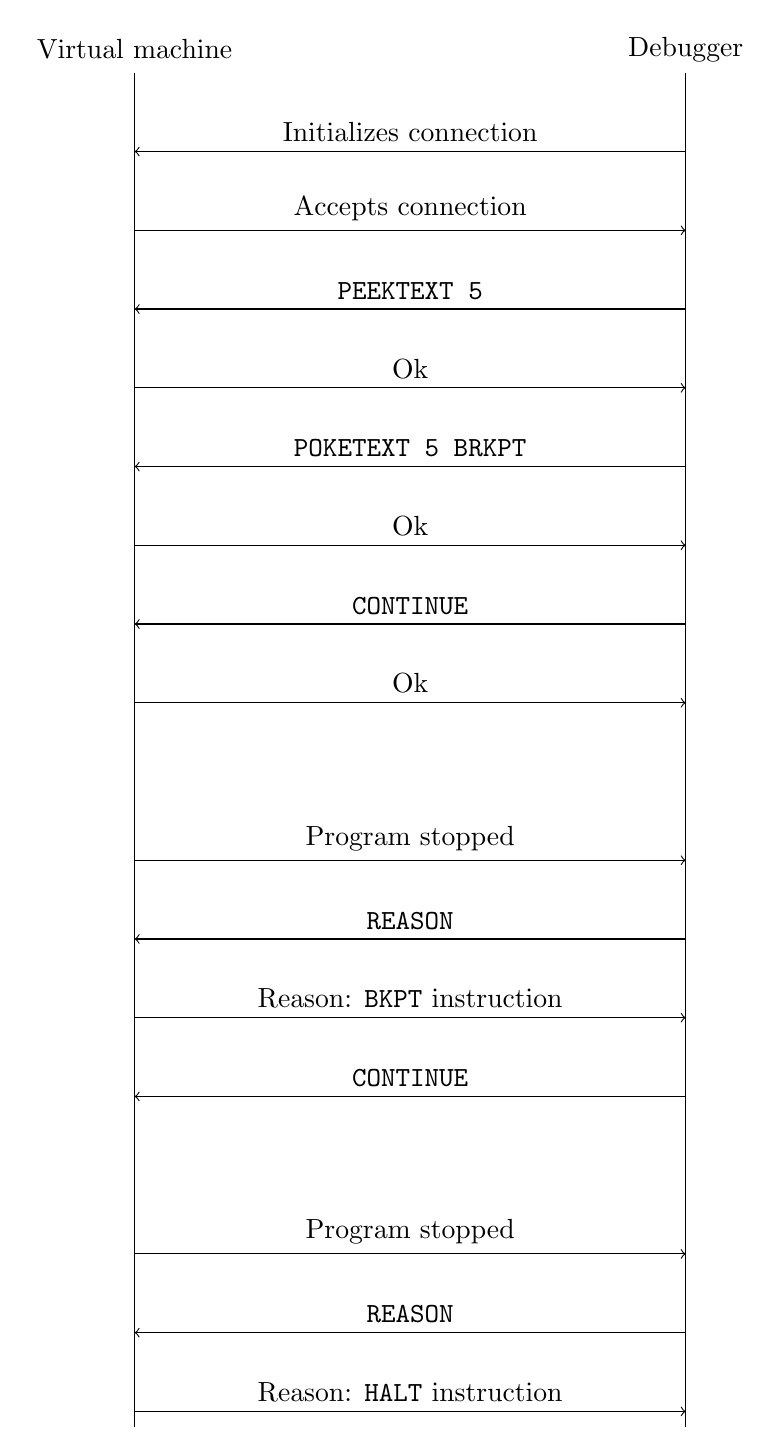
\begin{tikzpicture}
        \draw (0,0) -- (0,-17.2) (7,0) -- (7,-17.2);
        \node at (7,.3) {Debugger};
        \node at (0,.3) {Virtual machine};
        \draw[<-] (0,-1) -- node[midway,above] {Initializes connection} (7,-1);
        \draw[->] (0,-2) -- node[midway,above] {Accepts connection} (7,-2);
        \draw[<-] (0,-3) -- node[midway,above] {\texttt{PEEKTEXT 5}} (7,-3);
        \draw[->] (0,-4) -- node[midway,above] {Ok} (7,-4);
        \draw[<-] (0,-5) -- node[midway,above] {\texttt{POKETEXT 5 BRKPT}} (7,-5);
        \draw[->] (0,-6) -- node[midway,above] {Ok} (7,-6);
        \draw[<-] (0,-7) -- node[midway,above] {\texttt{CONTINUE}} (7,-7);
        \draw[->] (0,-8) -- node[midway,above] {Ok} (7,-8);
        \draw[->] (0,-10) -- node[midway,above] {Program stopped} (7,-10);
        \draw[<-] (0,-11) -- node[midway,above] {\texttt{REASON}} (7,-11);
        \draw[->] (0,-12) -- node[midway,above] {Reason: \texttt{BKPT} instruction} (7,-12);
        \draw[<-] (0,-13) -- node[midway,above] {\texttt{CONTINUE}} (7,-13);
        \draw[->] (0,-15) -- node[midway,above] {Program stopped} (7,-15);
        \draw[<-] (0,-16) -- node[midway,above] {\texttt{REASON}} (7,-16);
        \draw[->] (0,-17) -- node[midway,above] {Reason: \texttt{HALT} instruction} (7,-17);
    \end{tikzpicture}
    }
    \caption{A sequence diagram for the virtual machine and debugger communication.}
    \label{fig:dbg-vm-seq}
\end{figure}

\section{Native Debugger}
The implemented debugger has two main layers, first is to support native
instruction level debugging. This should work out of the box without any
debugging information whatsoever. The debugger has been implemented as a
library, inspired by LLDB. It is implemented in modern C++ up to the C++20
standard. The native debugger is also split into several layers to make it more
modular.

First layer is called \texttt{Process}, it is an interface. The implementation
of this interface is responsible for dealing with the concrete architecture,
the API of that architecture and the communication with the debuggee. One
implementation is provided for the T86 VM. For instance it has a method called
\texttt{ReadText} and \texttt{WriteText}. The internals of these methods use
the \texttt{PEEKTEXT} and \texttt{POKETEXT} API we described. Outside of this
class, the communication API is never used. If, in the future, another virtual
machine was made, for whichever architecture, it is only needed to implement
this interface. The rest of the debugger can be used as-is.

Another layer is the \texttt{Native} class. This implements the complicated
logic behind a debugger, like setting a breakpoint, handling singlestep and so
on. It is the main bread and butter of the native part of the debugger. Most of
the algorithms are similar to the linux debugger implementation presented in
section \todo{ref}. For illustration, in figure \ref{t86dbg:breakpoint} we show
a snippet of code that is used to create a breakpoint. It firstly reads the
text at address where we want to set the breakpoint. This text is then
rewritten by the breakpoint opcode and the backup is stored.

When we arrive at the breakpoint and want to continue further, we need to unset
the breakpoint, ie. replace the breakpoint opcode in the T86 program with the
backup we saved, do a native level single step, and write the breakpoint back.

Since breakpoints change the underlying code of the debuggee we need to be
careful when presenting information to the user. If we simply printed the text
that we get from the debuggee it might contain the \texttt{BKPT} instructions
we have set earlier. We need to mix it with the backup code stored in
breakpoints to correctly show the assembly of the program.

The Native class uses a \texttt{DebugEvent} structure which indicates what
caused the VM to stop. It is implemented as a \texttt{variant} of multiple
structures, for example \texttt{BreakpointHit}, \texttt{WatchpointTrigger} and
so on. The reason it is a variant is that because the watchpoint also needs to
convey information about an address that caused the break, same with the
breakpoint. It could also signal if the break was caused by reading or writing
to the memory cell, although for now the T86 VM only interrupts on writing.

\begin{figure}
    \begin{minted}{c++}
SoftwareBreakpoint CreateSoftwareBreakpoint(uint64_t address) {
    auto opcode = GetSoftwareBreakpointOpcode();
    // Read the text at the breakpoint address
    auto backup = process->ReadText(address, 1).at(0);
    // Rewrite it with the breakpoint opcode
    std::vector<std::string> data = {std::string(opcode)};
    process->WriteText(address, data);
    // Check that it was truly written
    auto new_opcode = process->ReadText(address, 1).at(0);
    if (new_opcode != opcode) {
        Error(...);
    }
    // Create a breakpoint object which keeps the text backup
    return SoftwareBreakpoint{backup, true};
}
    \end{minted}
    \caption{Debugger code in \texttt{Native} class to enable a breakpoint.}
    \label{t86dbg:breakpoint}
\end{figure}

As of now, the native debugger has following features:
\begin{itemize}
    \item Breakpoints - Can set, unset, enable and disable software breakpoints.
    \item Watchpoints - Can set and unset watchpoints on memory writes.
    \item Singlestep - Can do native level step into.
    \item Text manipulation - Can read and write into the debuggee text area,
        effectively allows to overwrite the running code.
    \item Data manipulation - Can read and write into the program RAM.
    \item Register manipulation - Can manipulate with normal, float and debug registers.
\end{itemize}

\section{Source debugger}
With the solid foundation represented by the native part of the debugger, we
can extend it by providing some form of source level debugging. For this part
we need to keep in mind that the debugger will only be used by students.
As such, we ought to have a gentler debugging information than DWARF,
but we certainly can take inspiration from it.

As we previously mentioned, the executable with T86 code is separated into sections.
The \texttt{.text} and \texttt{.data} sections are for the VM. We will introduce new
sections where debugging information will be stored. All those sections will have
\texttt{.debug\_} prefix. The simplest new section is \texttt{.debug\_source}, which
should contain the original source code which was compiled into this executable.
This later allows us, with combination of other information, to display the source
code lines where something abnormal happened.

The main philosophy of the source level debugger is to allow an arbitrary
amount of debug information. This means that an user can generate information
about one function only, and for that function source debugging capabilities
will work, but not for any other. This means that users can generate debug
information incrementally.

\subsection{Line information}
Line information is one of the simplest to generate. Since it'll probably be
the most generated information by the students, we choose the following simple
format for it: \texttt{<line>:<address>}. The section \texttt{.debug\_line} is
made up of these lines. The format is self explanatory, it says that line $x$
corresponds to address $y$. This is very easy to generate.

With this information, we are able to do source level breakpoints. If the
source code is also provided, we can show the user on which line is the
debugged program currently paused. It is not needed to specify every line in
the program. The debugger will simply refuse to put a source level breakpoint
on some line if it doesn't have the necessary information.

\subsection{Debugging information format}
In the line information, we provided a very easy format. However, to describe
some advanced constructs of the source, we will need an advanced structure.
Here we will draw inspiration from the Dwarf Debugging Information (DIE). Take
a look at figure \ref{fig:t86dbg-die}, which shows an example of such debugging
information. It has a tree like structure which in some ways mimics the
original program. The nodes of this tree are called debugging information
entries (DIEs). Those entries can have another entries as their children and
each entry has a tag which is part of its name (for example the
\texttt{compilation\_unit} tag). They can also have attributes which describe
their properties. As we can see, this is very similar to the DWARF entries.
This format is also a text one, this allows to generate the format easily and
also to easily find mistakes in it. We don't want to force the students to
debug their generated debugging information.

For instance, the function main has a name, a beginning address and end
address. Those two information are leveraged to allow setting breakpoints on
functions and also to display in which function are we currently located.
It also has a child, which is scope. Scope is mainly used for keeping
a track of which variables are currently active, because the T86 (or
any other assembly language in general) has no notion of scopes.
In the scope there is only one variable called \texttt{d}. Thanks to this,
we are able to list currently active variables.

\begin{figure}
    \begin{lstlisting}
DIE_compilation_unit: {
DIE_function: {
    ATTR_name: main,
    ATTR_begin_addr: 0,
    ATTR_end_addr: 10,
    DIE_scope: {
        ATTR_begin_addr: 0
        ATTR_begin_addr: 10
        DIE_variable: {
            ATTR_name: d,
        },
    }
}
}
    \end{lstlisting}
    \caption{Debugging function information for the T86 debugger.}
    \label{fig:t86dbg-die}
\end{figure}

It would however be much better if we could print their values and types. For
this, another piece of information is needed. We will introduce entries for
types. Currently, three type entries are present, one for primitive types (such
as int or float), one for pointers and one for structured types
(\texttt{struct} or \texttt{class} in C++). The types are saved as separate
entry, and as such we need some way to link them together with the variables.
To achieve this, we will use the \texttt{ATTR\_id} attribute. This attribute
should be unique for every entry. In this role it is similar to the id
attribute of HTML elements. The variables themselves have the \texttt{ATTR\_type}
attribute, which will have id of type as its value. An example of pointer type
which points to int is in figure \ref{fig:t86dbg-types}. If we had a variable
which is a pointer to int, it would need to have the \texttt{ATTR\_type: 1}
attribute, because id of pointer type to integer is one.

The primitive types need to have their size. For T86, this is the number of
memory cells it occupies, which will almost always be one, since one memory
cell is 64-bits. It also has a name of its primitive type. Currently, four are
supported: signed integer, unsigned integer, floating point number and a
boolean. The pointer type is simpler, it only needs its size (which again
is one for T86) and the id of type it points to.

Structured types are more complicated. They need to have a list of members
which are stored in the structure. For each of these members an offset
from the beginning of the structure must be specified as well. It also must
provide a size because the compiler might align it and it may be larger
than the sum of size of its members.

\begin{figure}
    \begin{lstlisting}
DIE_primitive_type: {
    ATTR_name: signed_int,
    ATTR_id: 0,
    ATTR_size: 1,
},
DIE_pointer_type: {
    ATTR_type: 1,
    ATTR_id: 1,
    ATTR_size: 1
},
    \end{lstlisting}
    \caption{Debugging type information for the T86 debugger.}
    \label{fig:t86dbg-types}
\end{figure}

With this information, we are able to show the type of the variable.
But the most valuable thing is its value. Variables either stored
in memory, register, or optimized out completely. We will go in
DWARF footsteps and provide a language for virtual machine that one
can interpret to gain the information.

A several examples can be seen in figure \ref{fig:t86dbg-vm}. Same as DWARF, it
is a stack based machine. The top value on the stack after computation is done
is considered to be the location of the variable. The instruction \texttt{PUSH}
pushes either offset or register onto the stack. The second example says that
the variable is located in register \texttt{R0}. The first example tells us
that the variable is in memory, at the address in register \texttt{BP} minus
two. The third example has the same meaning, but since the variables will
most often be stored at some offset from register \texttt{BP} a shorthand
was provided. There is also a dereference instruction, which can be used
to inspect to which location a pointer points.

\begin{figure}
    \begin{lstlisting}
- [PUSH BP; PUSH -2; ADD],
- `PUSH R0`
- `BASE_REG_OFFSET -2`
    \end{lstlisting}
    \caption{Debugging type information for the T86 debugger.}
    \label{fig:t86dbg-vm}
\end{figure}

This information is stored in a variable attribute called
\texttt{ATTR\_location}. Now we finally know where are some variables located
and might look up their value. Together with the type information, we might
also properly inspect the value and report it to the user. If no type
information is provided then the user is informed and the value is reprented as
raw bytes.

\subsection{Usage}
Finally, to make the debugger usable, we provide a command line interface which
leverages the debugger library. It provides many commands and its manual can be
found as appendix in this thesis.

The main priority of the CLI is to make the debugger easy to use. It consist of
several commands, one of them is \texttt{breakpoint set 5}, which will set a
source-level breakpoint on fifth line of the program. It is however not
necessary to write the whole command, any prefix will do, like \texttt{b s 5}.

The CLI also displays various information on program stop, like the reason why
the program stopped, on which address or line - if available, and also prints
the surrounding lines of assembly or source. The CLI can also list breakpoints
and display them straight in the disassembly or in the source view.

The whole project was done in the C++ language and some libraries were used to
make the implementation smoother. For example the famous \textit{fmt}
\todo{citace} library, which is used to format text with python like syntax.
Since we are working with text so much, it was a lifesaver. Another one is
\texttt{linenoise}, which we used to allow users to move back and forth in the
REPL when typing and also to have commands history. Another one is
\texttt{argparse}, used for parsing command line arguments and finally
\textit{GoogleTest}.

The debugger is of course not only limited to TinyC language. Any imperative
language that can be encoded with the debugging information we expect is
suitable to be debugged at source level. We show an example of this in a
provided test case for the CLI \todo{doplnit cestu}.

The repository is very well tested. It contains many unit tests for all parts
of the project, be it the T86 parser, the Native level debugging or the source
debugging. It also has an integration tests for the T86-CLI and the Debugger
CLI. The project itself was developed with the help of git and github has a
very describing development history via commit messages. A special care was
taken to ensure the main branch of the git repository always has a working
instance of the project. To this end the development was done via pull requests
and each request was merged if and only if all tests passed for it. Github issues
were used to track the current shortcomings of the project.
